\documentclass[12pt,a4paper]{article}
\usepackage[UTF8]{ctex}
\usepackage[backend=biber]{biblatex}
\usepackage{amsmath,amsthm,amssymb,graphicx,multirow,float,caption}
\usepackage{geometry}
\geometry{left=2.54cm, right=2.54cm, top=3.18cm, bottom=3.18cm}
\usepackage{enumitem}
\usepackage{subcaption,booktabs,diagbox}
\setenumerate[1]{itemsep=0pt,partopsep=0pt,parsep=\parskip,topsep=5pt}
\setitemize[1]{itemsep=0pt,partopsep=0pt,parsep=\parskip,topsep=5pt}
\setdescription{itemsep=0pt,partopsep=0pt,parsep=\parskip,topsep=5pt}
\usepackage{adjustbox}
\usepackage[graphicx]{realboxes}
\usepackage{rotating}

\usepackage{titlesec}

\titleformat{\section}%设置section的样式
{\raggedright\large\bfseries}%右对齐,4号字,加粗
{\thesection .\quad}%标号后面有个点
{0pt}%sep label和title之间的水平距离
{}%标题前没有内容

\title{\vspace{-4cm}\Large 光学多道与氢氘同位素光谱}  %文章标题
\author{\kaishu 学号:202111030007 \hspace{2cm} 姓名:郑晓旸}   %作者的名称
\date{\kaishu  实验日期: 2023年9月28日}

\begin{document}
\maketitle

\begin{abstract}
    本实验的目的是测量H原子和D原子在可见光波段内的几条谱线的波长值, 即电子从能级n=3,4,5,6到n=2跃迁时发出
    的光子的波长. 本实验使用光栅光谱仪进行测量, 使用两种类型的光电接收装置, 即基于光学多道的CCD和单色光电
    倍增管(PMT). 实验使用CCD测量了H原子和D原子典型谱线的波长, 使用PMT同样测量了谱线的波长, 
    还对400-660nm的氢氘同位素光谱整体进行了测量, 并得到了典型的谱线图. 基于谱线的波长测量, 得到了电子质子质量比, H和D原子的里德堡常数, 以及氢原子的能级图. 
    在做这些计算时, 一并进行了误差分析. 

    关键词: 氢氘同位素\ 里德堡常数\ 可见光波段
\end{abstract}

\section{引言}

用简短的语言介绍实验的相关背景(发展历程和前景、用途等)、实验目的等
物质的光谱与物质的组成的元素, 物质的微观构型决定的. 通过光谱分析, 能够获知物质的这些微观信息, 因此光谱学用途广泛. 
此外, 对基本元素的分析, 例如氢原子光谱的分析, 指导了20世纪量子力学的发展, 因而光谱学技术在物理学史中有着重要地位. 
特别地, 本实验将对氢氘同位素的光谱进行分析. 由于是气体发光, 光谱所呈现的只有原子信息. 通过对氢氘同位素的谱线间距测量, 能够了解
电子-质子质量比这一重要的原子微观参数. 


\section{原理}
在理解的基础上,用简明扼要的语言叙述实验原理,切忌照抄讲义

本实验的核心就是测量氢氘同位素的光谱. 特别地, 我们关注可见光波段内, 巴尔末线系n=3,4,5,6四条谱线的信息. 
实验仪器的主体是光栅光谱仪, 使用多色仪和单色仪两种光电转换方式进行谱线的测量. 

实验中使用的多色仪是光学多道分析仪, 一共2048道, 
每一道是由MOS制作的光电二极管作为感光像元, 每一道采集的波长为22nm. 因此使用光学多道分析仪时, 需要将待测谱线和标准谱线放在22nm的间隔内
进行测量. 

实验中使用的单色仪是光电倍增管. 单色仪的需要控制入射和出射的狭缝, 以保证测量的单色性. 在此基础上, 连续调整接收光栅出射光的平面镜转角, 
可以获得指定范围内的整个光谱. 

\section{实验}
介绍实验的仪器、实验方法和主要实验过程

\subsection{CCD}
实验中的标准谱线使用的是He灯和Ne灯. 其中Ne灯的标准谱线用于测量n=3的H-D同位素谱线, He灯的谱线用于测量n=4,5,6得到H-D同位素谱线. 

对每一条谱线的测量, 都大致分为如下几步: 

(1)调整中心波长至待测谱线附近. 

(2)调整H-D同位素仪的位置, 使得光线聚焦于入射光谱仪的狭缝处. 调整入射处狭缝的宽度, 直到仪器输出比较窄的峰. 

(3)通过剪除背景, 调节曝光等方式, 使得峰逐渐退化为双峰. 

(4)保存数据在寄存器1中. 关闭H-D同位素的光源. 
打开寄存器2, 换上He灯或Ne灯. 在另一个寄存器中调整灯的位置, 使得光线聚焦于入射狭缝处, 直到仪器输出三条标准谱线, 
且之前调出来的双峰也在附近. 

(5)根据三条标准谱线进行波长定标. 

(6)定出待测的两个峰的波长位置. 

\subsection{PMT}
PMT能够在指定波长区间内的每一波长进行测量, 因而能得到一个光源的可见光波段内的完整光谱. 这样的测量会在波长轴上
有一个未知的整体平移, 需要使用He的标准谱进行修正. 在测量H-D谱线时, 需要能够分辨相距很近的两个峰, 且由于随着n的增大
谱线的光强越来越小, 双峰的间距越来越近, 越来越以分辨, 因而需要仔细调整入射处和出射处的狭缝宽度, 以求能够分辨
波长最小的谱线, 即n=6, $\lambda \approx 410nm$的谱线. 

实验大致分为如下几个步骤: 
(1)调整狭缝的宽度, 使得在410nm处能够分辨H-D谱线的两个峰. 
(2)测量H-D同位素的整体光谱(400-660nm). 
(3)测量He灯的整体光谱(400-660nm).
(4)根据He灯的光谱进行波长修正. 
(5)使用扩展功能, 扩展H-D同位素光谱410nm, 430nm, 480nm, 655nm附近的双峰谱, 测量双峰的波长. 

\section{结果分析与讨论}
\subsection{CCD测量结果}
使用CCD进行的谱线测量, 是在408nm, 438nm, 497nm, 650nm为中心波长, 使用对应波长范围内的三条He灯和Ne灯(仅650nm处使用)标准谱进行定标的.
定标后测量的数据, 和理论计算值的比较如表\ref{Char1}:  
\begin{table}[H]
    \centering
    \begin{tabular}{|c|c|c|c|c|c|c|}
    \hline
        & $D_{\text{测量}}$      & $D_{\text{理论}}$      & $\Delta \lambda_{D} $ & $H_{\text{测量}}$      & $H_{\text{理论}}$     & $\Delta \lambda_{H} $  \\ \hline
    n=3 & 656.10 & 656.294 & 0.194 & 656.27 & 656.473 & 0.203 \\ \hline
    n=4 & 486.05 & 486.143 & 0.093 & 486.17 & 486.276 & 0.106 \\ \hline
    n=5 & 433.98 & 434.057 & 0.059 & 434.11 & 434.175 & 0.065 \\ \hline
    n=6 & 410.01 & 410.183 & 0.182 & 410.07 & 410.296 & 0.226 \\ \hline
    \end{tabular}
    \caption{使用CCD对氢氘同位素n=3,4,5,6的谱线波长测量及与理论值的对比(单位:nm).
    其中$\Delta \lambda=\lambda_{\text{理论}}-\lambda_{\text{测量}}$.}
    \label{Char1}
    \end{table}

定标的原理是用标准谱线拟合一个线性函数, 使用该函数对标准谱线的测量结果如下:

可以看出: (1)波长的绝对测量的误差相对于理论值的偏差在0.1-0.2nm左右 (2)氢氘相同能级的谱线间距与理论间距的差距
$\delta \lambda=\Delta \lambda_{H}-\Delta \lambda_{D}$的值在0.01-0.05nm. 这表明在同一个定标标准下, 尽管波长的绝对值不准确, 但测量的间距相对准确. 
也就是说, 双峰相对于理论值的误差大致相同, 考虑到它们的间距本来就比较小, 这个结果并不意外. 

为了进一步分析误差的来源, 我们呈现使用标准谱线进行定标得到的拟合函数对标准谱线测量的结果,如表\ref{Char2}: 

\begin{table}[H]
    \centering
    \begin{tabular}{|c|c|c|c|}
    
    \hline
    n=3 & 650.66 & 653.28 & 659.90 \\ \hline
    $Ne_{\text{标}}$  & 656.65 & 653.29 & 659.90 \\ \hline
    n=4 & 492.19 & 501.55 & 504.78 \\ \hline
    $He_{\text{标}}$  & 492.19 & 501.57 & 504.77 \\ \hline
    n=5 & 438.79 & 443.74 & 447.14 \\ \hline
    $He_{\text{标}}$  & 438.79 & 443.74 & 447.15 \\ \hline
    n=6 & 402.62 & 412.07 & 414.37 \\ \hline
    $He_{\text{标}}$  & 402.62 & 412.08 & 414.38 \\ \hline
    \end{tabular}
    \caption{使用标准谱线定标的拟合函数对标准谱线的测量结果(单位:nm).其中每两行中第一行是测量值, 第二行是标准光源的谱线值}
    \label{Char2}
    \end{table}

可以看到, 定标带来的误差在0nm-0.02nm. 前述对波长的绝对大小的测量误差($\sim 0.1nm$)远远大于这一值, 因而我们认为该误差是一种系统误差. 
注意到衍射方程
\begin{equation}
    d\sin{\theta}=m \lambda
\end{equation}
其中d是光栅常数, m是衍射级数, $\theta$是以中心波长为基准的波长为$\lambda$的谱线的衍射角的位置. 
在使用线性拟合近似时, 会背离正弦曲线, 偏离的程度取决于$\theta$的值, 或者说待测波长与中心波长的间隔. 

除了这个系统误差以外, 另一个可能的误差来自于噪声. 如下图中410nm附近, n=6的双峰图,如图\ref{fig1}: 
\begin{figure}[H]
    \centering
    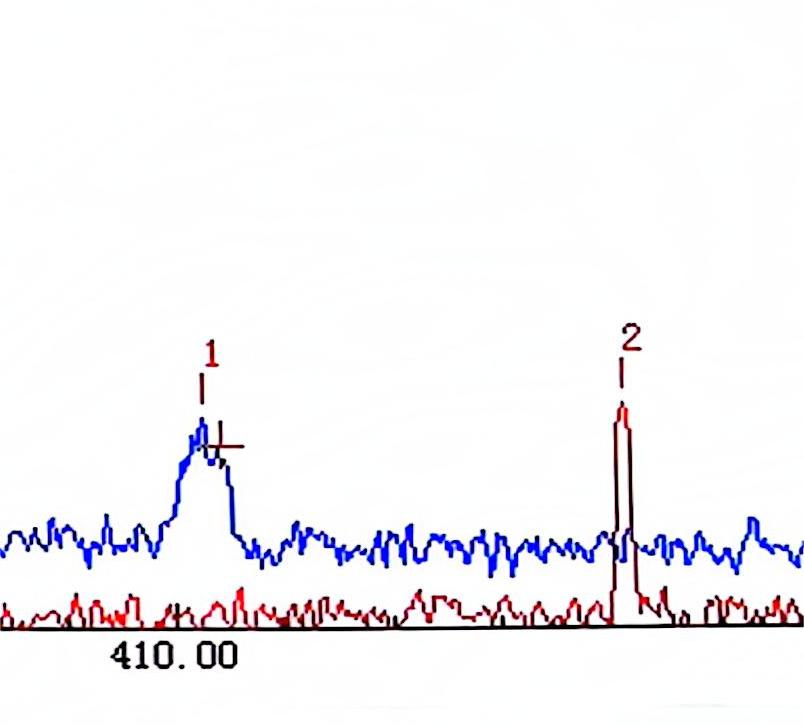
\includegraphics[width=0.5\textwidth]{CCD 410.jpg}
    \caption{CCD测量的n=6处的H-D双峰谱线(蓝). 其中右边红色的峰是He灯标准谱线412.08nm. }
    \label{fig1}
\end{figure}
可见, 由于n=6的谱线强度和噪声拉不开明显差距, 噪声很容易改变双峰的位置, 尤其是光强较小的那个峰. 这导致双峰的标定有较大误差.

\subsection{PMT测量结果}
通过调整入射处和出射处的狭缝宽度, 在410nm附近分辨出来双峰以后, 扫描测量400-660nm的谱线。得到可以同时分辨$n=3,4,5,6$的所有H-D双峰的谱。根据PMT扫描得到的数据,绘制谱线图\ref{fig2}如下:
\begin{figure}[htbp]
    \centering
    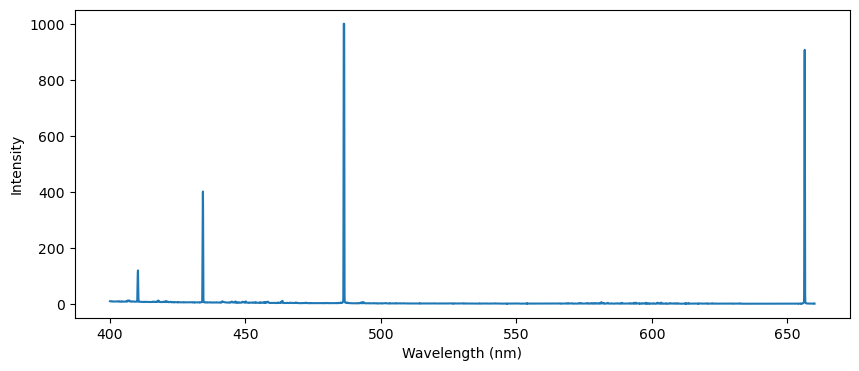
\includegraphics[width=0.7\textwidth]{PMT.png}
    \caption{PMT测量的H-D同位素光谱}
    \label{fig2}
\end{figure}
\\
放大后, 分别在待测谱线附近进行扩展, 得到下面的四张图\ref{fig3}, \ref{fig4}, \ref{fig5}, \ref{fig6}:
\begin{figure}[htbp]
	\centering
	\begin{minipage}{0.49\linewidth}
		\centering
		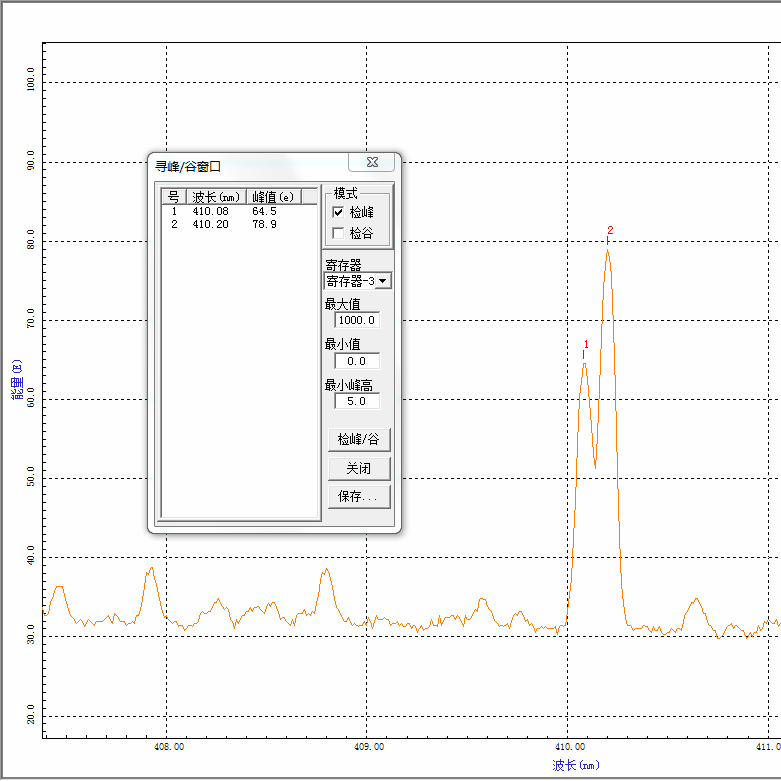
\includegraphics[width=0.9\linewidth]{HD_408_412.png}
		\caption{PMT测量410nm双峰}
		\label{fig3}
	\end{minipage}
	\begin{minipage}{0.49\linewidth}
		\centering
		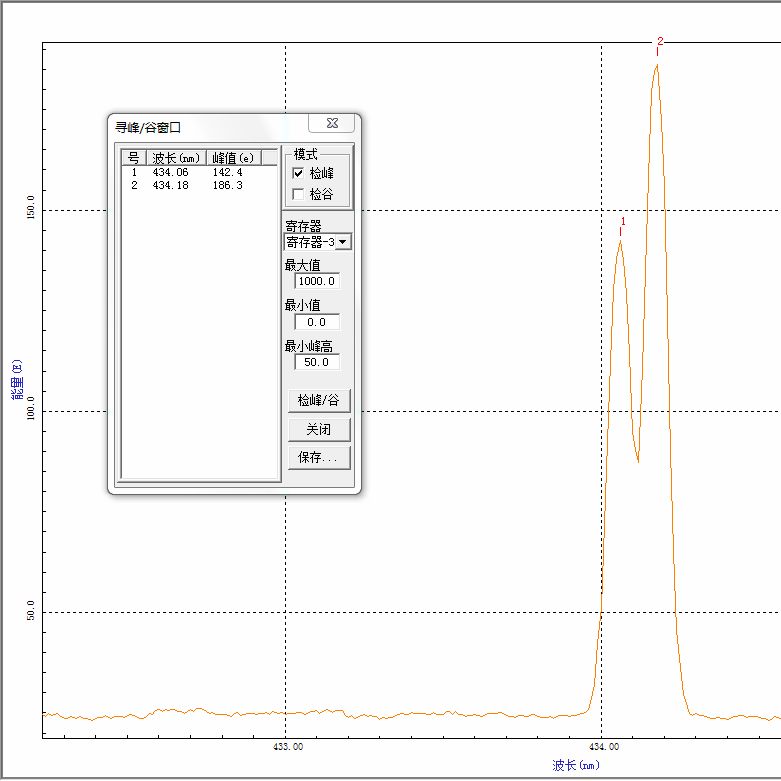
\includegraphics[width=0.9\linewidth]{HD_433_435.png}
		\caption{PMT测量434nm双峰}
		\label{fig4}
	\end{minipage}
	%\qquad
	%让图片换行,
	\\
	\begin{minipage}{0.49\linewidth}
		\centering
		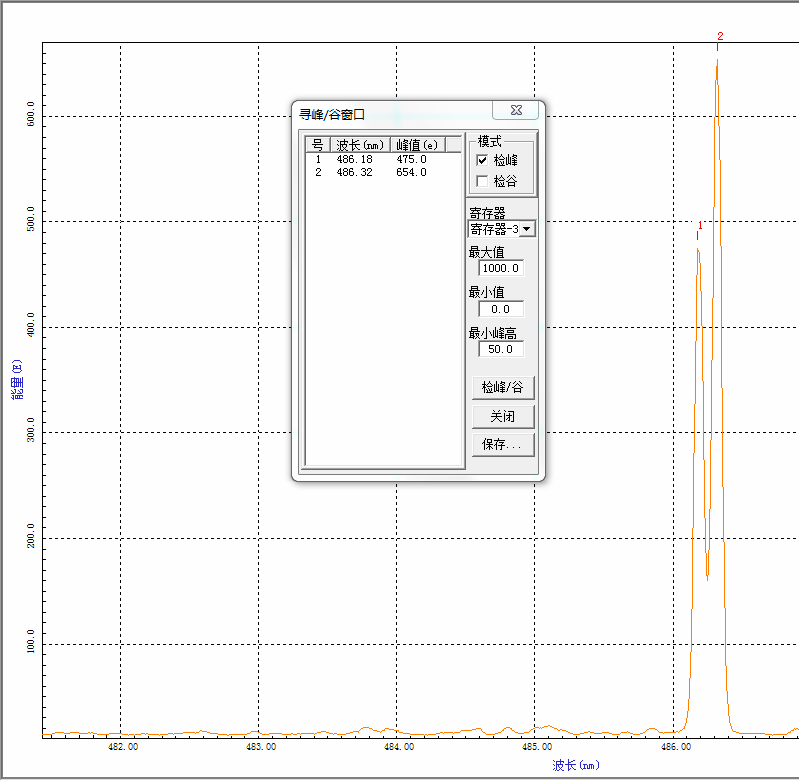
\includegraphics[width=0.9\linewidth]{HD_485_487.png}
		\caption{PMT测量486nm双峰}
		\label{fig5}
	\end{minipage}
	\begin{minipage}{0.49\linewidth}
		\centering
		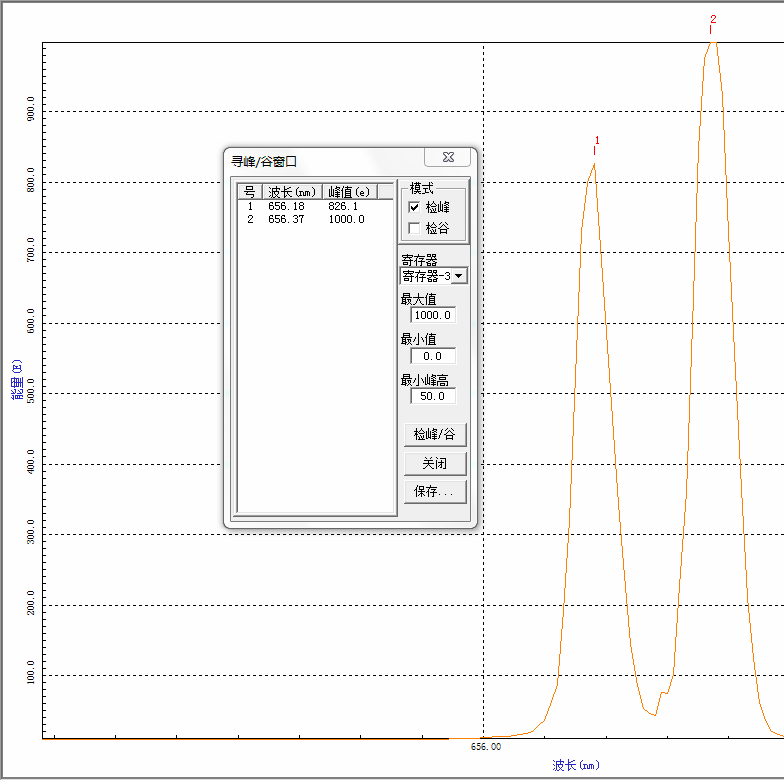
\includegraphics[width=0.9\linewidth]{HD_656_657.png}
		\caption{PMT测量656nm双峰}
		\label{fig6}
	\end{minipage}
\end{figure}
图中除了呈现双峰的谱线以外, 还呈现了使用寻峰功能对波长进行测量的过程. 

与CCD中一样, 对n=3,4,5,6的巴尔末线系氢氘同位素谱线波长值与理论值的对比如下表\ref{Char3}: 
\begin{table}[H]
    \centering
    \begin{tabular}{|c|c|c|c|c|c|c|}
    \hline
        & $D_{\text{测量}}$      & $D_{\text{理论}}$      & $\Delta \lambda_{D} $ & $H_{\text{测量}}$      & $H_{\text{理论}}$     & $\Delta \lambda_{H} $  \\ \hline
    n=3 & 656.18 & 656.294 & -0.114 & 656.37 & 656.473 & -0.103 \\ \hline
    n=4 & 485.18 & 486.143 & 0.037 & 486.32 & 486.276 & 0.044 \\ \hline
    n=5 & 434.06 & 434.057 & 0.051 & 434.18 & 434.175 & 0.005 \\ \hline
    n=6 & 410.08 & 410.183 & 0.103 & 410.20 & 410.296& 0.096 \\ \hline
    \end{tabular}
    \label{Char3}
    \caption{使用PMT对氢氘同位素n=3,4,5,6的谱线波长测量及与理论值的对比(单位:nm).
    其中$\Delta \lambda=\lambda_{\text{测量}}-\lambda_{\text{理论}}$.}
    \end{table}
整体的误差相较于CCD的测量来说小了一个量级. 但是由于PMT的波长定标并不是基于拟合函数, 而只能通过对He标准谱线个别谱线的修正来进行整体平移. 所以, 并不是
考虑了He的所有标准谱线来求出一个合适的平移量, 因此会带来一定误差. n=3,6的误差比其他几个显著地大, 可能就是这个原因. 

\subsection{计算里德伯常数$R_{H}$和$R_{D}$}
使用巴尔末公式
\begin{equation}
    \frac{1}{\lambda}=R_{X}(\frac{1}{2^2}-\frac{1}{n^2})
\end{equation}
该公式利用里德伯常数$R_{X}$计算电子从能级n跃迁回能级n=2时发出的光子的波长. 

根据公式
\begin{equation}
    R_{\mathrm{H}}=R_{\infty} \frac{m_{\mathrm{p}}}{m_{\mathrm{p}}+m_{\mathrm{e}}}, \quad R_{\mathrm{D}}=R_{\infty} \frac{2 m_{\mathrm{p}}}{2 m_{\mathrm{p}}+m_{\mathrm{e}}}
\end{equation}

代入$R_{\infty}=109737.31 cm^{-1}$, 计算得到:
\begin{equation}
    R_{\mathrm{H}}=109677.58cm^{-1}, \quad R_{\mathrm{D}}=109707.44cm^{-1}
\end{equation}
    
计算里德伯常数使用的方法是正比例拟合$y=kx$, 其中x取n=3,4,5,6时的离散值$\frac{1}{2^2}-\frac{1}{n^2}$, y是$\frac{1}{\lambda}$. k就是待拟合的里德堡
常数$R_{X}$. 使用mathematica内置函数NonlinearModelFit进行拟合. 我们先用表1或表3中的标准波长进行拟合, 以验证这种方法的可靠性.

\begin{table}[H]
    \centering
    \begin{tabular}{|c|c|c|c|c|}
    \hline
       & Estimate & Standard Error & t-Statistic                   & P-Value                         \\ \hline
    $R_{H}$ & 109677   & 0.0437482      & $2.50701*10^6$ & $1.3996*10^{-19}$  \\ \hline
    $R_{D}$  & 109707   & 0.0593884      & $1.84728*10^6$ & $3.49842*10^{-19}$ \\ \hline
    \end{tabular}
    \caption{使用标准波长进行的拟合. 数据源: Mathematica中内置函数NonlinearModelFit的ParameterTable}.
    \end{table}

可见, 拟合的值与理论计算值是对的上的, 且标准差的量级在$10^{-2}$. 

下面来看用CCD测量得到的结果, 计算出来的里德堡常数: 

\begin{table}[H]
    \centering
    \begin{tabular}{|c|c|c|c|c|}
    \hline
       & Estimate & Standard Error & t-Statistic & P-Value                         \\ \hline
    $R_{H}$ & 109704   & 1.69425        & 64750.5     & $8.12346*10^{-15}$ \\ \hline
    $R_{D}$ & 109729   & 3.88277        & 28260.4     & $9.77089*10^{-14}$ \\ \hline
    \end{tabular}
    \caption{使用CCD测量的波长进行的拟合. 数据源: Mathematica中内置函数NonlinearModelFit的ParameterTable}.
    \end{table}

CCD的测量结果与标准值相差$20cm^{-1}$, 标准差在$5cm^{-1}$的量级. 

下面是使用PMT测量得到的结果, 计算出来的里德堡常数: 

\begin{table}[H]
    \centering
    \begin{tabular}{|c|c|c|c|c|}
    \hline
      & Estimate & Standard Error & t-Statistic & P-Value                         \\ \hline
      $R_{H}$ & 109690   & 10.1694        & 10786.3     & $1.75733*10^{-12}$ \\ \hline
      $R_{D}$  & 109721   & 10.3876        & 10562.7     & $1.87132*10^{-12}$ \\ \hline
    \end{tabular}
    \caption{使用PMT测量的波长进行的拟合. 数据源: Mathematica中内置函数NonlinearModelFit的ParameterTable}.
    \end{table}

PMT的测量结果与标准值相差$10cm^{-1}$, 标准差在$10cm^{-1}$的量级. 这个量级比CCD测量的更大, 反映了PMT测量在精确度方面的方差更大(n=3,6时比其他n大的误差). 

需要注意, 前面用CCD和PMT测量时, 分析得到的由各种各样的原因造成的波长测量误差为$\delta \lambda=0.1nm$的量级, 由于$\frac{1}{\lambda}\propto R_{X}$, 有
\begin{equation}
    \delta R_{X}=R_{X}*\vert\frac{\delta \lambda}{\lambda}\vert \approx 109700 cm^{-1} *\frac{0.1}{500}\approx 20 cm^{-1}
\end{equation}

拟合出来的结果与理论值的偏差, 确实在这个量级. 

此外, 由于空气的折射率n=1.00027, 造成的相对误差仅有0.027\%, 对本节结论影响不大. 
\subsection{计算电子-质子质量比}
下面计算电子-质子质量比. 主要到公式: 
\begin{equation}
    \frac{\delta \lambda}{\lambda_{D}} \approx \frac{m_{e}}{2 m_{p}}
\end{equation}

我们先计算标准值: 
\begin{equation}
    \frac{m_{e}}{2 m_{p}}=5.44617*10^{-4}
\end{equation}

下面仍然使用拟合的方法进行计算. 使用的拟合函数是$y=kx$, 其中y是$\Delta  \lambda$, x是$\lambda_{D}/2$, 这样k就是待求的电子-质子质量比. 
先使用标准波长计算, 拟合结果如下: 
\begin{table}[H]
    \centering
    \begin{tabular}{|c|c|c|c|c|}
    \hline
      & Estimate    & Standard Error                 & t-Statistic & P-Value                        \\ \hline
    $\frac{me}{mp}$ & 0.000546448 & $1.32353*10^{-6}$ & 412.872     & $3.13339*10^{-8}$ \\ \hline
    \end{tabular}
    \caption{使用标准波长计算的电子-质子质量比}
    \end{table}

可见, 已经与标准值发生偏离, 偏离的量级正好是标准差的量级$10^{-6}$. 可见, 要比较好的计算电子质子质量比, 需要更多的波长有效位数, 
本实验显然做不到这一点. 

下面是使用CCD测量的波长计算的结果: 
\begin{table}[H]
    \centering
    \begin{tabular}{|c|c|c|c|c|}
    \hline
      & Estimate   & Standard Error & t-Statistic & P-Value    \\ \hline
      $\frac{me}{mp}$ & 0.00049037 & 5.45791E-05    & 8.98457     & 0.00291032 \\ \hline
    \end{tabular}
    \caption{使用CCD测量的波长计算的电子-质子质量比}
    \end{table}

CCD测量的结果相对误差已经达到了10\%, 与理论值的差距也在10\%.

下面是使用PMT测量的波长计算的结果:
\begin{table}[H]
    \centering
    \begin{tabular}{|c|c|c|c|c|}
    \hline
      & Estimate    & Standard Error & t-Statistic & P-Value    \\ \hline
      $\frac{me}{mp}$ & 0.000490324 & 5.45665E-05    & 8.98579     & 0.00290918 \\ \hline
    \end{tabular}
    \caption{使用PMT测量的波长计算的电子-质子质量比}
    \end{table}

PMT测量的结果与CCD相似, 相对误差已经达到了10\%, 与理论值的差距也在10\%.

为了解释这个结果, 取波长测量的不确定度$u(\lambda)=0.1nm$, $u(\delta \lambda)=0.05nm$(可见4.1中分析). 

使用下述公式, 以n=4为例, 进行不确定度的计算, 有: 
\begin{equation}
u(W)=\sqrt{\sum_{i=1}^{N}\left(u\left(x_{i}\right) \frac{\partial W}{\partial x_{i}}\right)^{2}}
\end{equation}
得到$u(me/mp)=1.5*10^{-4}$. 

前面拟合的结果比这个估计要好一些, 应当是统计平均的缘故. 

\subsection{氢原子能级}
以$-\overline R_{H}/n^2$为纵轴绘制的氢原子能级图如下所示. 图中还标注了各跃迁及对应波长. 
\begin{figure}[H]
    \centering
    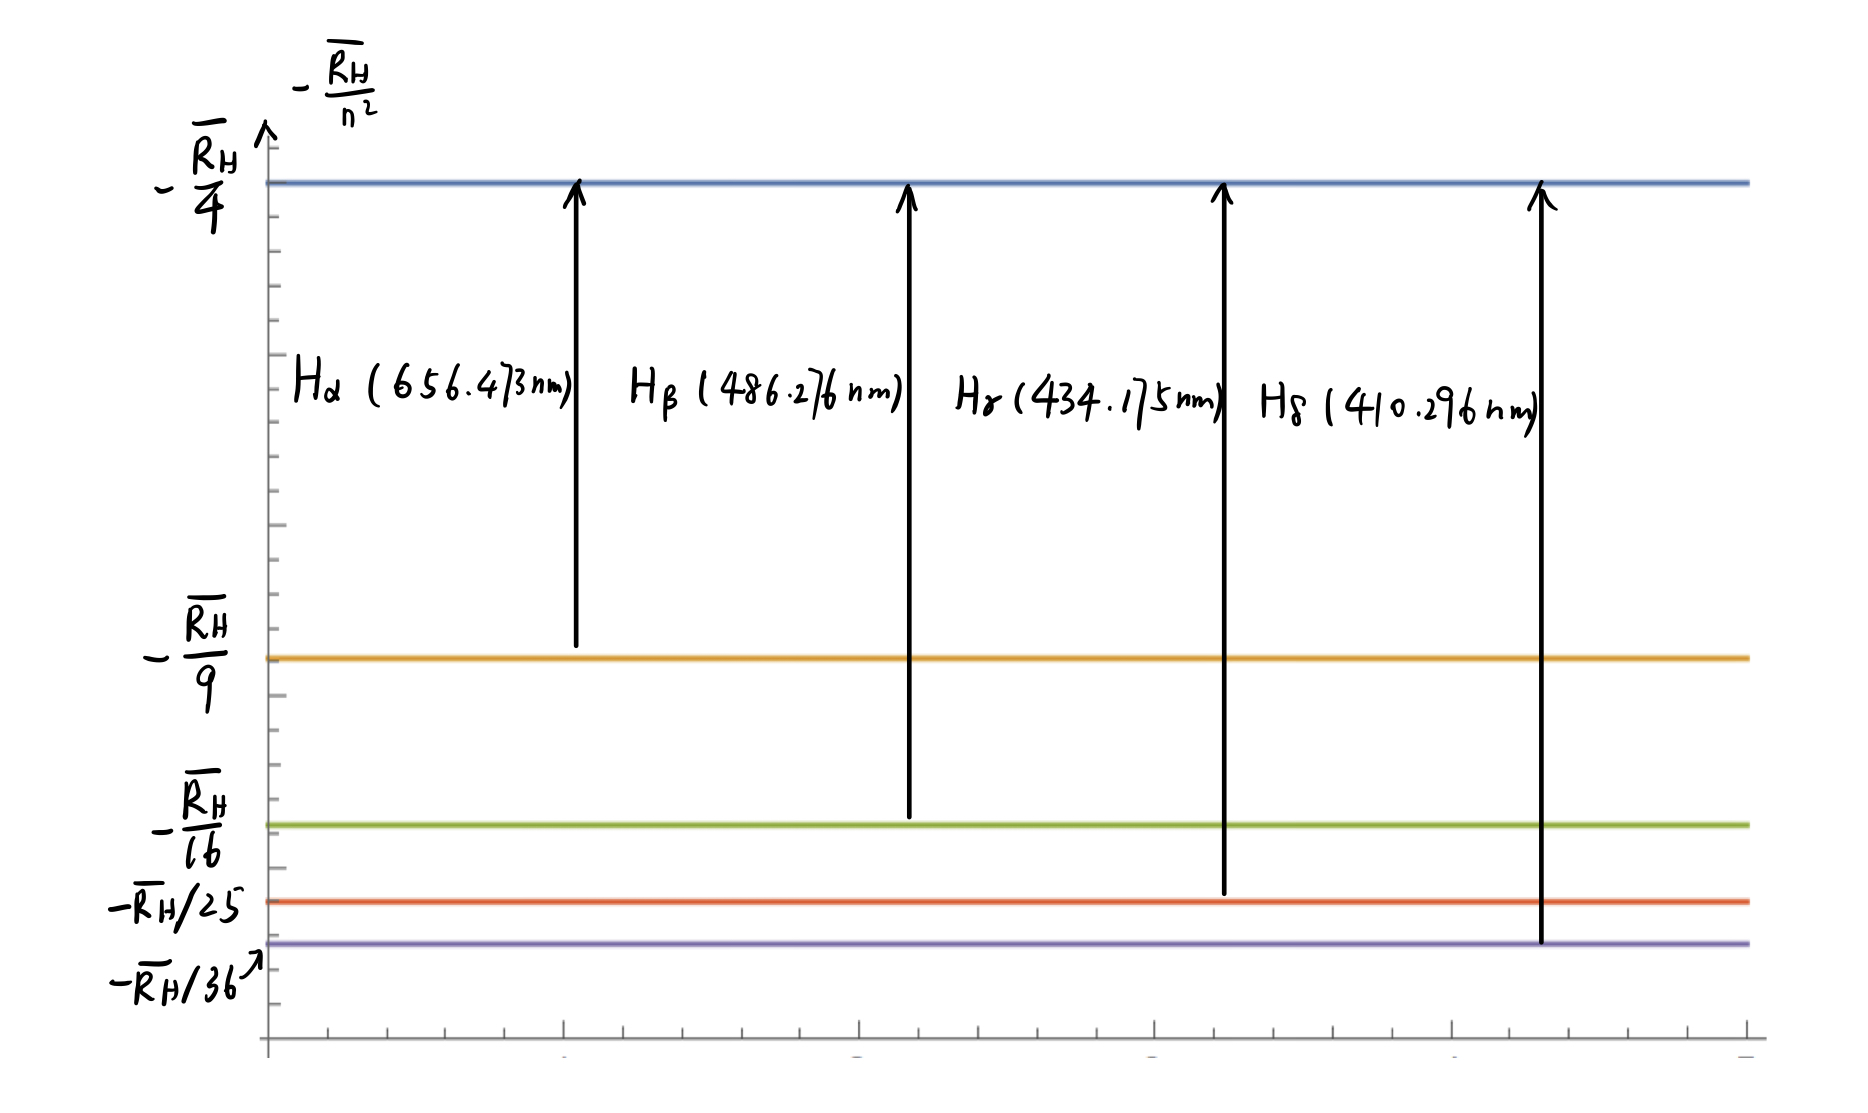
\includegraphics[width=0.9\textwidth]{氢原子能级.jpg}
    \caption{氢原子能级图}
\end{figure}


\subsection{H-D同位素光源400nm-660nm整体光谱}
\begin{figure}[H]
    \centering
    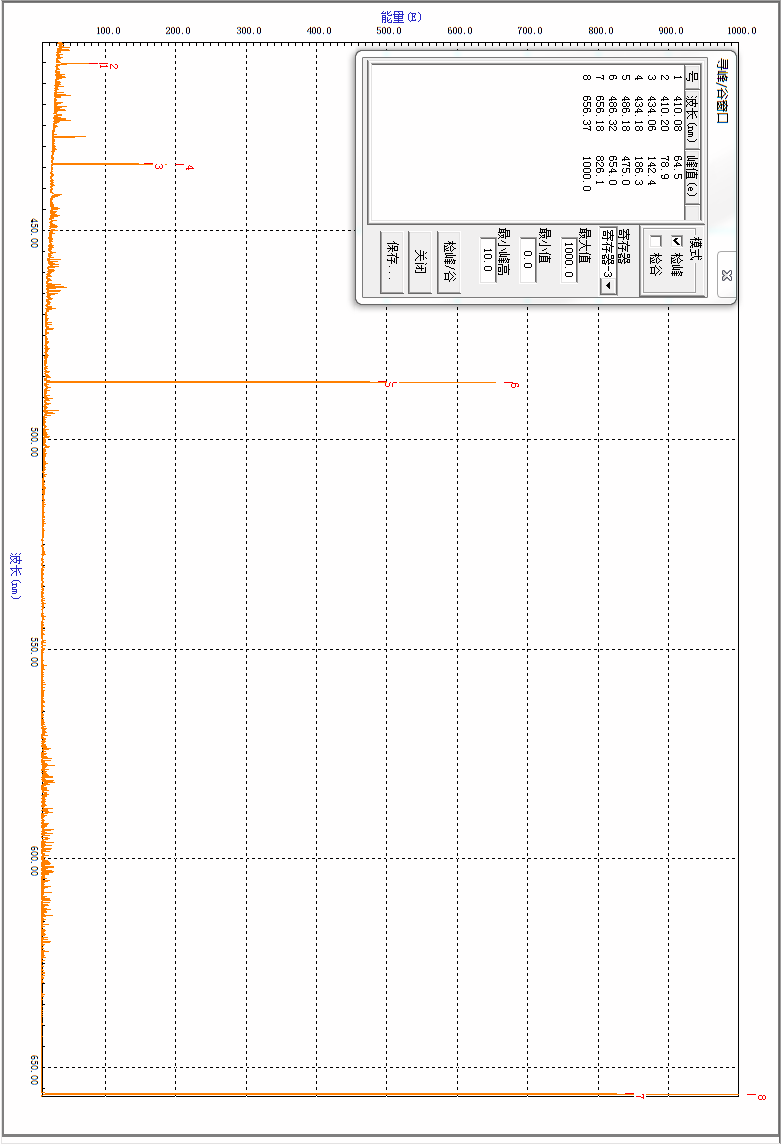
\includegraphics[width=0.8\textwidth]{HD_407-667.png}
    \caption{H-D同位素光源400nm-660nm整体光谱}
\end{figure}


\section{总结}
本实验使用CCD和PMT两种方法对氢氘同位素仪的光谱进行了测量. 测量得到了可见光波段巴尔末线系n=3,4,5,6的波长值. 
利用这些波长值, 进行了里德堡常数, 电子质子质量比的计算. 此外, 在使用PMT的过程中, 还输出了氢氘同位素仪在434nm附近n=5的波谱扩展图, 以及400nm-660nm的
完整波谱. 
\section{附录: 原始实验数据}
\begin{figure}[H]
    \centering
    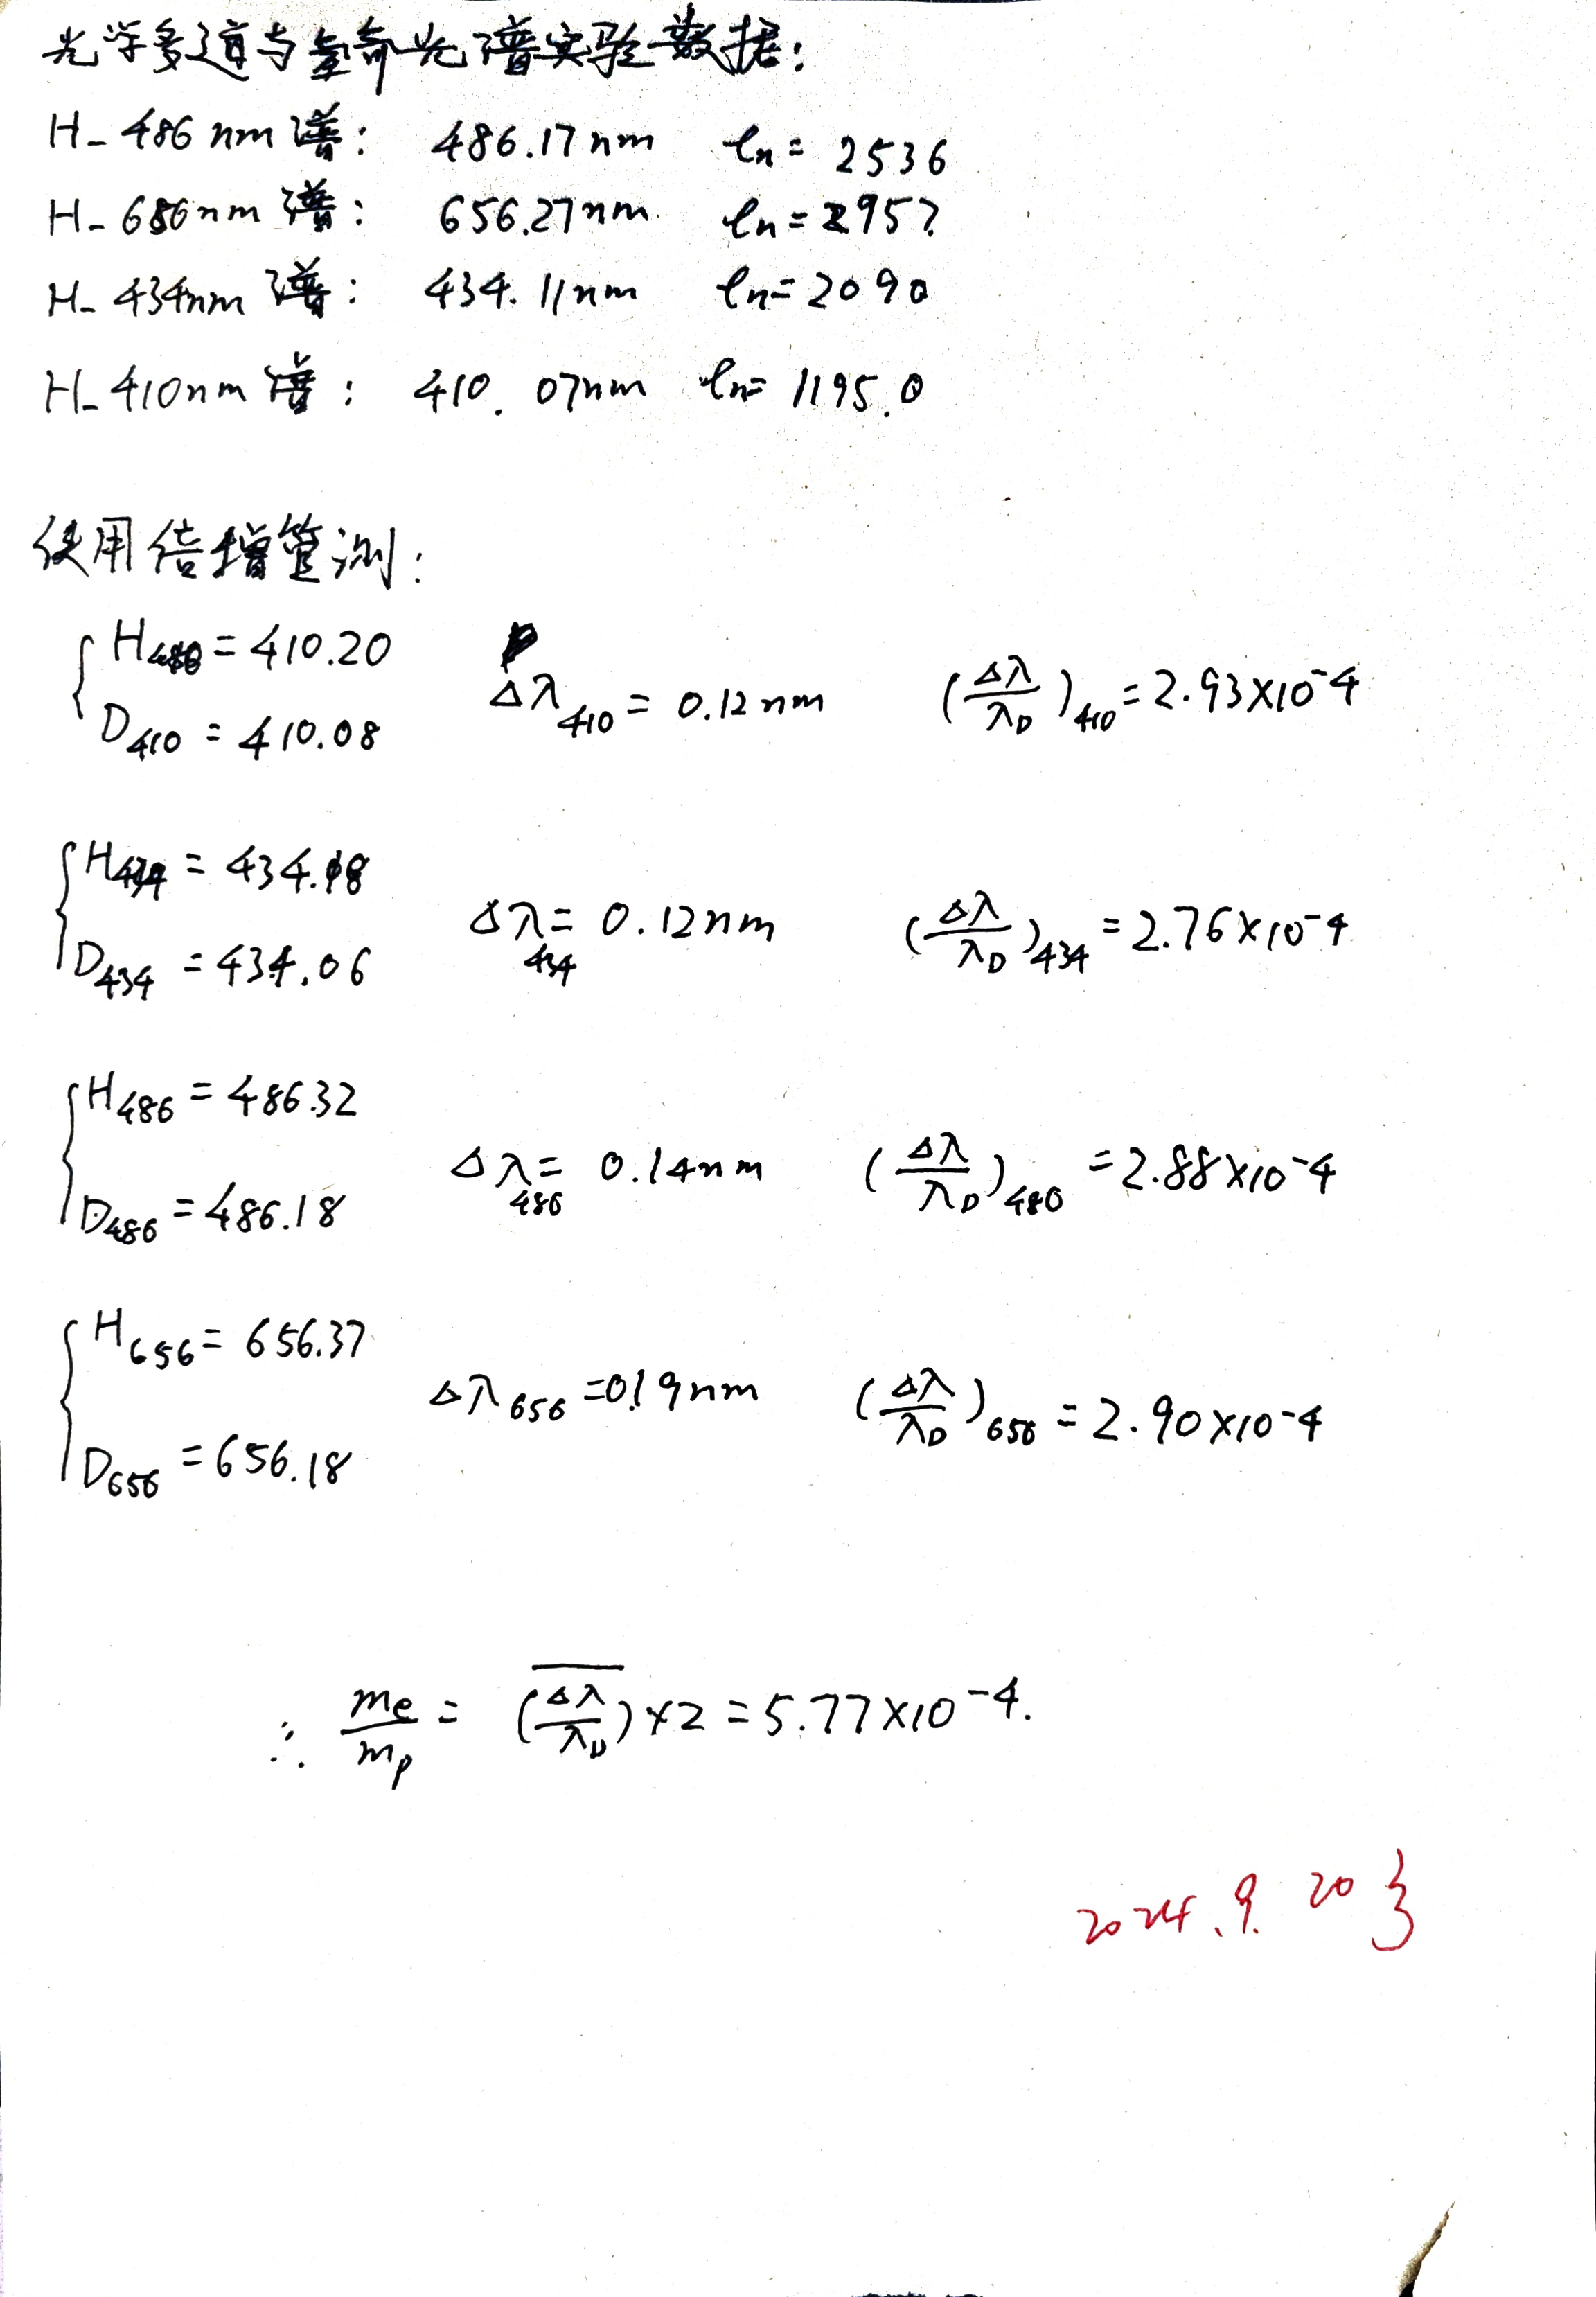
\includegraphics[width=0.5\textwidth]{Appendix.jpg}
\end{figure}
\end{document}